\documentclass[a4paper,12pt]{article}
\usepackage[utf8]{inputenc} % Ensure the file is saved with UTF-8 encoding
\usepackage[T1]{fontenc}
\usepackage[spanish]{babel}  % Para escribir en español
\usepackage[a4paper, margin=1in]{geometry}
\usepackage{graphicx}  % Para insertar imágenes
\usepackage{geometry}  % Para ajustar los márgenes
\usepackage{titling}   % Para personalizar el título
\usepackage{setspace}  % Para ajustar el espaciado
\usepackage{fancyhdr}
\usepackage{xcolor}    % Para cambiar el color de la línea del encabezado
\usepackage{listings}
\usepackage{soul}
\usepackage{caption}
\usepackage{wrapfig}
\usepackage{longtable}  % Para dividir en varias páginas
\usepackage{float}  % Ayuda con los entornos flotantes
\usepackage[absolute,overlay]{textpos}
\usepackage[hidelinks]{hyperref}
\geometry{top=2cm,bottom=2cm,left=2cm,right=2cm}  % Márgenes personalizados

\definecolor{mybeige}{RGB}{245, 245, 200}
\definecolor{lightblue}{RGB}{173, 216, 230}
\definecolor{lightgray}{RGB}{240, 240, 240}

% Configuración del encabezado
\pagestyle{fancy}
\fancyhf{}
\fancyhead[L]{
\includegraphics[height=1.5cm]{Imagenes/logounex.png}}  % Imagen a la izquierda
\fancyhead[C]{\raisebox{0.3cm}{\shortstack{Programación en Bases de Datos \\ Proyecto Hacking Ético: SQL Injection}}}  % Texto en el centro
\fancyhead[R]{
\includegraphics[height=1.5cm]{Imagenes/logopoli.png}}  % Imagen a la derecha
\renewcommand{\headrulewidth}{0.4pt}  % Línea debajo del encabezado
\setlength{\headheight}{1.5cm}
\setlength{\headsep}{1cm}
\setlength{\TPHorizModule}{1cm}
\setlength{\TPVertModule}{1cm}

% Configuración del pie de página
\fancyfoot[L]{\textit{Universidad de Extremadura}}  % Texto a la izquierda
\fancyfoot[C]{\thepage}  % Número de página en el centro
\fancyfoot[R]{\textit{Curso 2024-2025}}  % Texto a la derecha
\renewcommand{\footrulewidth}{0.4pt}  % Línea encima del pie de página
\setlength{\footskip}{0cm}

% Configuración del entorno listings para resaltar el código Python
\lstset{
    inputencoding=utf8,
    language=Python,
    basicstyle=\ttfamily\small,
    backgroundcolor=\color{mybeige},
    keywordstyle=\color{blue},
    commentstyle=\color{green},
    stringstyle=\color{red},
    frame=single,
    rulecolor=\color{black},
    showstringspaces=false,
    numbers=left,
    numberstyle=\tiny,
    numbersep=5pt,
    tabsize=4,
    breaklines=true,
    breakatwhitespace=false,
    escapeinside={(*@}{@*)},
    literate={ñ}{{\~n}}1
             {á}{{\'a}}1
             {é}{{\'e}}1
             {í}{{\'i}}1
             {ó}{{\'o}}1
             {ú}{{\'u}}1
             {Á}{{\'A}}1
             {É}{{\'E}}1
             {Í}{{\'I}}1
             {Ó}{{\'O}}1
             {Ú}{{\'U}}1
             {Ñ}{{\~N}}1
}

\lstset{
    language=SQL, % Utiliza SQL como base
    basicstyle=\ttfamily\small,
    backgroundcolor=\color{mybeige},
    keywordstyle=\color{blue}\bfseries,
    commentstyle=\color{green!50!black},
    stringstyle=\color{red},
    frame=single,
    rulecolor=\color{black},
    showstringspaces=false,
    numbers=left,
    numberstyle=\tiny,
    numbersep=5pt,
    tabsize=4,
    breaklines=true,
    breakatwhitespace=false,
    escapeinside={(*@}{@*)},
    morekeywords={
        PROCEDURE, FUNCTION, BEGIN, END, DECLARE, IF, THEN, ELSE, ELSIF, 
        LOOP, FOR, WHILE, EXIT, NULL, EXCEPTION, RAISE, COMMIT, ROLLBACK,
        CURSOR, OPEN, FETCH, CLOSE, GRANT, REVOKE, PACKAGE, TYPE, 
        ALTER, DROP, TRUNCATE, MERGE, USING, VALUES, INTO, SELECT, 
        INSERT, UPDATE, DELETE, RETURN, OUT, IN, INOUT, CONSTANT
    },
    morecomment=[l]{--}, % Comentarios de una línea con --
    morecomment=[s]{/*}{*/}, % Comentarios de bloque
    morestring=[b]', % Cadenas entre comillas simples
    inputencoding=utf8,
    literate={ñ}{{\~n}}1
             {á}{{\'a}}1
             {é}{{\'e}}1
             {í}{{\'i}}1
             {ó}{{\'o}}1
             {ú}{{\'u}}1
             {Á}{{\'A}}1
             {É}{{\'E}}1
             {Í}{{\'I}}1
             {Ó}{{\'O}}1
             {Ú}{{\'U}}1
             {Ñ}{{\~N}}1
}

\lstdefinestyle{console}{
    backgroundcolor=\color{lightgray}, % Color de fondo
    basicstyle=\ttfamily\small,        % Fuente monoespaciada y tamaño pequeño
    breaklines=true,                   % Permitir saltos de línea
    stringstyle=\color{black},
    frame=single,                      % Marco alrededor del código
    framerule=0.5pt,                   % Grosor del marco
    rulecolor=\color{black},           % Color del marco
    xleftmargin=0.5cm,                 % Margen izquierdo
    xrightmargin=0.5cm,                % Margen derecho
    aboveskip=1em,                     % Espacio antes del bloque
    belowskip=1em,                     % Espacio después del bloque
    escapeinside={(*@}{@*)},
    inputencoding=utf8,      % Configura el encoding
    literate={ñ}{{\~n}}1
             {á}{{\'a}}1
             {é}{{\'e}}1
             {í}{{\'i}}1
             {ó}{{\'o}}1
             {ú}{{\'u}}1
             {Á}{{\'A}}1
             {É}{{\'E}}1
             {Í}{{\'I}}1
             {Ó}{{\'O}}1
             {Ú}{{\'U}}1
             {Ñ}{{\~N}}1
}

\begin{document}

\begin{titlepage}
    \centering

    % Imagen de la portada (fotoportada)
    
\includegraphics[width=0.75\textwidth]{Imagenes/fotoportada.png} % Asegúrate de que el archivo esté en la misma carpeta

    \vspace{1cm}

    % Título
    {\Huge \textbf{Programación en Bases de Datos} \par}

    \vspace{0.3cm}

    % Línea de separación
    \rule{\linewidth}{0.1mm}

    \vspace{0.3cm}

    % Subtítulo
    {\LARGE \textbf{Proyecto Hacking Ético: SQL Injection} \par}

    \vspace{1.5cm}

    % Logo de la universidad (logounex)
    
\includegraphics[width=0.25\textwidth]{Imagenes/logounex.png} % Asegúrate de que el archivo esté en la misma carpeta

    \vfill

    % Autor
    {\footnotesize Alejandro Bofill Gonzalez - David Gordillo Burrero - Aarón Manzano Mateos - Ángel Macías Barro \par}

\end{titlepage}

\newpage

\begin{center}
    \renewcommand{\contentsname}{Índice de contenidos}\tableofcontents
\end{center}

\newpage

%Introduccion
\section{Introducción al proyecto}
El presente documento aborda el tema del hacking ético y su aplicación en el estudio de vulnerabilidades en bases 
de datos, con un enfoque particular en las inyecciones SQL. Estas vulnerabilidades constituyen uno de los riesgos 
más comunes y críticos en aplicaciones web que interactúan con bases de datos, permitiendo a los atacantes manipular 
o acceder a información de manera no autorizada. Este trabajo tiene como propósito profundizar en la comprensión de las 
inyecciones SQL, analizando sus tipos, los riesgos asociados y los motivos por los cuales ocurren, para fomentar una perspectiva 
integral de la seguridad en el desarrollo de software.
\vspace{0,5cm}
Para facilitar el aprendizaje práctico y la evaluación de estas vulnerabilidades, se ha desarrollado un laboratorio interactivo 
basado en tecnologías como Flask y Python. Este entorno de simulación permite experimentar con diferentes tipos de inyecciones SQL,
 ofreciendo a los usuarios una experiencia inmersiva y controlada. El laboratorio incluye aplicaciones web diseñadas específicamente
  para emular escenarios reales de inyecciones SQL, permitiendo realizar pruebas tanto en bases de datos Oracle como en PostgreSQL.
   Estas bases de datos, seleccionadas por su relevancia y amplio uso en entornos empresariales, proporcionan un contexto diverso y
    representativo para explorar las técnicas de ataque y sus consecuencias.
    \vspace{0,5cm}

Cada tipo de inyección SQL implementada en el laboratorio ha sido cuidadosamente seleccionada para cubrir un amplio espectro de 
vulnerabilidades. Entre ellas, se encuentran las inyecciones basadas en errores, que explotan los mensajes de error generados por
 la base de datos para extraer información sensible; las inyecciones de tipo "Union Attack", que utilizan la cláusula UNION para 
 combinar resultados de consultas y obtener datos confidenciales; las inyecciones basadas en booleanos, que permiten inferir 
 información mediante la manipulación de condiciones lógicas; y las inyecciones ciegas, que aprovechan diferencias en el 
 comportamiento de la aplicación para deducir detalles de la base de datos sin generar mensajes de error explícitos.
 \vspace{0,5cm}

El diseño del laboratorio incluye páginas individuales para cada tipo de inyección, con formularios de inicio de sesión 
vulnerables, credenciales específicas para realizar las pruebas y explicaciones detalladas sobre el ataque correspondiente.
 Esto permite que los usuarios comprendan tanto la teoría subyacente como la ejecución práctica de cada tipo de inyección. 
 Además, el laboratorio cuenta con documentación complementaria que explica cómo se implementaron las vulnerabilidades y su 
 relevancia en entornos reales, proporcionando una base sólida para que los participantes puedan identificar y mitigar estos 
 riesgos en sus propios proyectos.

 \vspace{0,5cm}
Este trabajo no solo subraya los riesgos asociados con las inyecciones SQL, como el acceso no autorizado a datos confidenciales,
 la alteración o eliminación de información crítica y el compromiso total del servidor de base de datos, sino que también explora 
 las causas más comunes detrás de estas vulnerabilidades. Entre ellas, se encuentran la falta de sanitización de las entradas del
  usuario, el uso de consultas dinámicas inseguras y la ausencia de auditorías de seguridad durante el desarrollo de software. Al
   comprender estos factores, se busca fomentar la adopción de mejores prácticas en la construcción de aplicaciones seguras y
    resilientes.
    
    \vspace{0,5cm}
En conclusión, este proyecto combina un enfoque teórico y práctico para abordar una de las amenazas más relevantes 
en el ámbito de la seguridad informática. Al proporcionar un entorno interactivo y educativo, se espera que este laboratorio 
no solo aumente la conciencia sobre la importancia de prevenir las inyecciones SQL, sino que también capacite a los participantes
 en la identificación, explotación controlada y mitigación de estas vulnerabilidades. Este esfuerzo refleja el compromiso con la 
 promoción de un desarrollo de software más seguro, alineado con los principios del hacking ético y la ciberseguridad.

 \section{Inyección SQL}

    \subsection{¿Qué es una inyección SQL?}

 Imagina que estás en un restaurante y entregas tu orden al mesero. Si todo funciona como debería, el mesero simplemente transmite tu pedido al chef, quien prepara la comida según lo solicitado. Ahora bien, ¿qué pasaría si, en lugar de un pedido normal, decides escribir en la nota algo como: "Quiero una pizza, y además dame acceso a la caja registradora"? Si el sistema del restaurante no tiene medidas para validar las órdenes, es posible que el mensaje llegue al chef, quien podría malinterpretarlo como una instrucción válida y permitirte hacer algo que no deberías poder hacer. Algo similar ocurre con una inyección SQL, pero en el contexto de aplicaciones web y bases de datos.
 \vspace{0,5cm}

 Una inyección SQL es un tipo de ataque en el que un atacante manipula las consultas que una aplicación web hace a su base de datos para ejecutar comandos maliciosos. Esto sucede cuando el sistema no valida adecuadamente las entradas proporcionadas por los usuarios y las trata directamente como parte de la consulta SQL. Por ejemplo, en una página de inicio de sesión, si un usuario malintencionado introduce un texto diseñado específicamente para alterar la lógica de la consulta SQL que valida las credenciales, podría obtener acceso no autorizado al sistema sin necesidad de conocer la contraseña.
 \vspace{0,5cm}

 Un caso real que ilustra el impacto de las inyecciones SQL ocurrió en el año 2012, cuando un grupo de atacantes explotó esta vulnerabilidad en una aplicación de LinkedIn. Mediante una inyección SQL, los atacantes lograron acceder a información confidencial de usuarios, incluidos datos de inicio de sesión. Este incidente no solo expuso la información personal de millones de personas, sino que también dañó la reputación de la compañía y resaltó la gravedad de no implementar medidas de seguridad adecuadas.
 \vspace{0,5cm}

 Por ejemplo, imagina una consulta SQL en una aplicación web que maneja la autenticación de usuarios. Una consulta típica podría ser:
 \vspace{0,2cm}

 \begin{lstlisting}[language=SQL]
SELECT * FROM usuarios 
WHERE nombre_usuario = 'usuario' 
AND contraseña = 'contraseña';
 \end{lstlisting}
 \vspace{0,2cm}

 Si el sistema permite que un atacante ingrese algo como \texttt{usuario' OR '1'='1} en lugar del nombre de usuario, la consulta resultante sería:
 \vspace{0,2cm}

 \begin{lstlisting}[language=SQL]
SELECT * FROM usuarios 
WHERE nombre_usuario = 'usuario' OR '1'='1' 
AND contraseña = 'contraseña';
\end{lstlisting}
\vspace{0,2cm}

 La condición \texttt{'1'='1'} siempre es verdadera, lo que significa que el atacante podría acceder al sistema sin necesidad de proporcionar credenciales válidas. Este ejemplo muestra cómo una entrada maliciosa puede alterar la lógica de una consulta SQL, dándole al atacante el control.
 \vspace{0,5cm}

 Las inyecciones SQL pueden tener consecuencias graves, que incluyen el robo de datos confidenciales, la modificación o eliminación de registros, y en casos extremos, el control total del servidor de la base de datos. Además, son una de las vulnerabilidades más comunes en aplicaciones web, según el \textit{OWASP} (Open Web Application Security Project). Sin embargo, prevenirlas no es complicado si se aplican prácticas adecuadas, como el uso de consultas preparadas, la validación estricta de entradas y la implementación de controles de acceso robustos.
 \vspace{0,5cm}

 En resumen, una inyección SQL no es solo un fallo técnico, sino un ejemplo de cómo pequeñas omisiones en la seguridad pueden tener grandes repercusiones. Conocer cómo ocurren y cómo prevenirlas es esencial para cualquier profesional que desarrolle aplicaciones conectadas a bases de datos, ya que no solo se trata de proteger sistemas, sino también la confianza y la información de los usuarios.
 
 \subsection {Causa principal de las inyecciones SQL}


%Preparacion del entorno explicacion de las funciones de requerimientos
\section{Preparación del entorno}
En este apartado se detallarán los requerimientos necesarios para la correcta ejecución del proyecto, 
así como las funciones que se han implementado para la creación de la base de datos y la inserción de datos en la misma.

\subsection{Prerequisitos}
A modo de base para el correcto desarrollo y ejecución del proyecto, es necesario tener instalado en el sistema los siguientes paquetes:
\begin{itemize}
    \item Oracle Database
    \item PostgreSQL Database
    \item Python 
\end{itemize}

La version descargada de los anteriores paquetes puede ser la que ha sido configurada en anteriores prácticas 
desarrolladas en la asignatura de Programación en Bases de Datos.

\subsection{Requerimientos de ejecución}
Una vez configurados correctamente los prerequisitos que no estan ligados especificamente con esta práctica,
se procederá a la instalación de las librerias y frameworks de python que han sido necesarios para el desarrollo de este laboratorio.
Para facilitar este proceso se ha generado un fichero con las librerias necesarias que se puede instalar mediante el siguiente comando:

\begin{lstlisting}[style=console]
    pip install -r requirements.txt
\end{lstlisting}

En dicho fichero \textit{requirements.txt} se encuentran las siguientes librerias:
\begin{itemize}
    \item \textbf{Flask} con version 2.2.0
    \item \textbf{werkzeug} con version 2.2.0
    \item \textbf{oracledb} con version mayor o igual a 2.4.1
    \item \textbf{psycopg2} con version mayor o igual a 2.9.9
    \item \textbf{requests} con version mayor o igual a 2.32.2
    \item \textbf{termcolor} con version 2.2.0
    \item \textbf{yaspin} con version mayor o igual a 3.1.0
\end{itemize}

\section{Conexión de la base de datos}
Para la conexión de la base de datos se han implementado funciones de conectar y desconectar que permiten la conexión a Oracle y PostgreSQL.
Estas funciones se han implementado en los archivos \textit{setupOracle.py} y \textit{setupPostgres.py}.
A continuación se detallan las funciones implementadas en cada uno de los archivos.

\subsection{Oracle}
A continuación se muestran las funciones que se ha implementado en el archivo \textit{setupOracle.py} para la conexión a Oracle.

\begin{lstlisting}[language=Python]
# Función para conectar a la base de datos
def dbConectarOracle():
    ip = "localhost"
    puerto = 1521
    s_id = "xe"
    usuario = "system"
    contrasena = "12345"

    print("---dbConectarOracle---")
    print("---Conectando a Oracle---")

    try:
        conexion = PBD.connect(user=usuario, password=contrasena, host=ip, port=puerto, sid=s_id)
        print("Conexión realizada a la base de datos", conexion)
        return conexion
    except PBD.DatabaseError as error:
        print("Error en la conexión")
        print(error)
        return None

# Función para desconectar de la base de datos
def dbDesconectar(conexion):
    print("---dbDesconectar---")
    try:
        if conexion:  # Verifica que la conexión no sea None
            conexion.commit()  # Confirma los cambios

            conexion.close()
            print("Desconexión realizada correctamente")
            return True
        else:
            print("No hay conexión para cerrar.")
            return False
    except PBD.DatabaseError as error:
        print("Error en la desconexión")
        print(error)
        return False
\end{lstlisting}

\subsection{PostgreSQL}
A continuación se muestra la funciones que se ha implementado en el archivo \textit{setupPostgres.py} para la conexión a PostgreSQL.

\begin{lstlisting}
    
def dbConectarPostgreSQL():
ip = "localhost"
puerto = 5432
basedatos = "Empresa"

usuario = "postgres"
contrasena = "12345"

print("---dbConectarPostgreSQL---")
print("---Conectando a Postgresql---")

try:
    conexion = PBD.connect(user=usuario, password=contrasena, host=ip, port=puerto, database=basedatos)
    print("Conexión realizada a la base de datos",conexion)
    return conexion
except PBD.DatabaseError as error:
    print("Error en la conexión")
    print(error)
    return None

#-------------------------------------------------------------------

def dbDesconectar(conexion):
print("---dbDesconectar---")
try:
    conexion.commit()  # Confirma los cambios
    conexion.close()
    print("Desconexión realizada correctamente")
    return True
except PBD.DatabaseError as error:
    print("Error en la desconexión")
    print(error)
    return False
\end{lstlisting}
%Setup Oracle y Setup Postgre
\section{Creación de tablas}
Para la creación de las tablas en Oracle y PostgreSQL se han implementado dos funciones que permiten la creación de las mismas.
Se ha decidido crear una tabla llamada \textit{Usuarios} con los campos \textit{id}, \textit{username}, \textit{password} y \textit{session\_cookie}.
Además, se ha incluido la inserción de usuarios de ejemplo en la tabla, para poder hacer uso de ellos en las inyecciones del laboratorio.
Estas funciones se han implementado en los archivos \textit{setupOracle.py} y \textit{setupPostgres.py}. 
A continuación se detallan las funciones implementadas en cada uno de los archivos.

\subsection{Oracle}
A continuación se muestra la función que se ha implementado en el archivo \textit{setupOracle.py} para la creación de la tabla en Oracle.
\begin{lstlisting}[language=Python]
    # Funcion para la configuracion de tablas
    def configuracionTablas\_oracle(conexion):
        print("---configuracionTablas---")
        try:
            cursor = conexion.cursor()
    
            # Crear tabla Usuarios si no existe con columna session\_cookie
            consulta = """
                BEGIN
                    EXECUTE IMMEDIATE 'CREATE TABLE Usuarios (
                        id NUMBER GENERATED BY DEFAULT AS IDENTITY PRIMARY KEY,
                        username VARCHAR2(50) NOT NULL UNIQUE,
                        password VARCHAR2(50) NOT NULL,
                        session\_cookie VARCHAR2(255)
                    )';
                EXCEPTION
                    WHEN OTHERS THEN
                        IF SQLCODE = -955 THEN
                            NULL;  -- Ignora si la tabla ya existe
                        ELSE
                            RAISE;
                        END IF;
                END;
            """
            cursor.execute(consulta)
    
            # Insertar usuarios de ejemplo solo si la tabla esta vacia
            cursor.execute("SELECT COUNT(*) FROM Usuarios")
            count = cursor.fetchone()[0]
            print("Usuarios en la tabla:", count)
            if count == 0:
                usuarios\_ejemplo = [
                    ("admin", "password123", "t4SpnpWyg76A3K2BqcFh2vODq0fqJGvs38ydh9"),
                    ("user1", "password1", "d382yd8n21df4314fn817yf6834188ls023d8d"),
                    ("user2", "password2", "u73dv226d726gh23fnjncuyg0q9udfjf47eueu")
                ]
                cursor.executemany(
                    "INSERT INTO Usuarios (username, password, session\_cookie) VALUES (:username, :password, :session\_cookie)",
                    usuarios\_ejemplo
                )
                print("Usuarios de ejemplo insertados correctamente.")
            else:
                print("La tabla Usuarios ya contiene datos.")
    
            cursor.close()
            print("Tabla 'Usuarios' creada o verificada exitosamente")
            return True
        except PBD.DatabaseError as error:
            print("Error al crear la tabla o insertar usuarios")
            print(error)
            return False
\end{lstlisting}

\subsection{PostgreSQL}
A continuación se muestra la función que se ha implementado en el archivo \textit{setupPostgres.py} para la creación de la tabla en PostgreSQL.
\begin{lstlisting}[language=Python]
def configuracion_tablas_postgresql(conexion):
print("---configuracion_tablas_postgresql---")
try:
    cursor = conexion.cursor()

    # Crear la tabla Usuarios si no existe con columna session_cookie
    consulta = """
        CREATE TABLE IF NOT EXISTS Usuarios (
            id SERIAL PRIMARY KEY,
            username VARCHAR(50) NOT NULL UNIQUE,
            password VARCHAR(50) NOT NULL,
            session_cookie VARCHAR(255)
        );
    """
    cursor.execute(consulta)

    # Insertar usuarios de ejemplo solo si la tabla esta vacia
    cursor.execute("SELECT COUNT(*) FROM Usuarios")
    count = cursor.fetchone()[0]
    if count == 0:
        usuarios_ejemplo = [
            ("admin", "password123", "t4SpnpWyg76A3K2BqcFh2vODq0fqJGvs38ydh9"),
            ("user1", "password1", "d382yd8n21df4314fn817yf6834188ls023d8d"),
            ("user2", "password2", "u73dv226d726gh23fnjncuyg0q9udfjf47eueu")
        ]
        cursor.executemany(
            "INSERT INTO Usuarios (username, password, session_cookie) VALUES (%s, %s, %s)",
            usuarios_ejemplo
        )
        print("Usuarios de ejemplo insertados correctamente.")
    else:
        print("La tabla Usuarios ya contiene datos.")

    cursor.close()
    print("Tabla 'Usuarios' creada o verificada exitosamente en PostgreSQL")
    return True
except PBD.DatabaseError as error:
    print("Error al crear la tabla o insertar usuarios en PostgreSQL")
    print(error)
    return False
\end{lstlisting}


%Introducción laboratorio explicando en detalle cada funcion
\section{Introducción al laboratorio}
Se ha desarrollado un laboratorio interactivo que permite experimentar con diferentes tipos de inyecciones SQL en bases de datos Oracle y PostgreSQL. 
En los siguientes apartados se explicará en detalle cada inyección y cómo se ha implementado en el laboratorio.

%Documentacion inyeccion a inyeccion (otra \section separada)
\section(Inyección basada en errores de la base de datos)
La \textbf{inyección SQL basada en errores} es un tipo de ataque de inyección SQL en el que el atacante explota la información 
expuesta directamente por los mensajes de error generados por la base de datos. Estos mensajes de error proporcionan pistas sobre la estructura, 
el esquema y el contenido de la base de datos, lo que permite al atacante ejecutar consultas maliciosas para obtener acceso no autorizado 
a los datos o comprometer la integridad del sistema.

\subsection{Mecanismo del Ataque}

\begin{itemize}
    \item \textbf{Explotación de Mensajes de Error:}
    Durante el desarrollo de aplicaciones web, los desarrolladores suelen habilitar mensajes de error detallados para depurar problemas. 
    Si estos mensajes no se desactivan en producción, los atacantes pueden intencionalmente introducir consultas mal formadas o comandos SQL 
    en los puntos de entrada de la aplicación (por ejemplo, formularios o parámetros URL) para provocar errores.

    \item \textbf{Uso de Consultas Maliciosas:}
    El atacante inserta código SQL diseñado para causar un error deliberado y obtener un mensaje detallado de la base de datos. 
    Estos mensajes pueden revelar información sensible como nombres de tablas, nombres de columnas, tipos de datos o incluso fragmentos del 
    contenido almacenado.

    \item \textbf{Iteración del Proceso:}
    Basándose en los datos recopilados de los mensajes de error, el atacante ajusta y refina sus consultas maliciosas para extraer información 
    adicional o lograr un acceso más profundo al sistema.
\end{itemize}

Para acceder a la sección especifica para esta inyección en el laboratorio, una vez desplegado el servidor con una apariencia como la siguiente:

\begin{figure}[H]
    \centering
    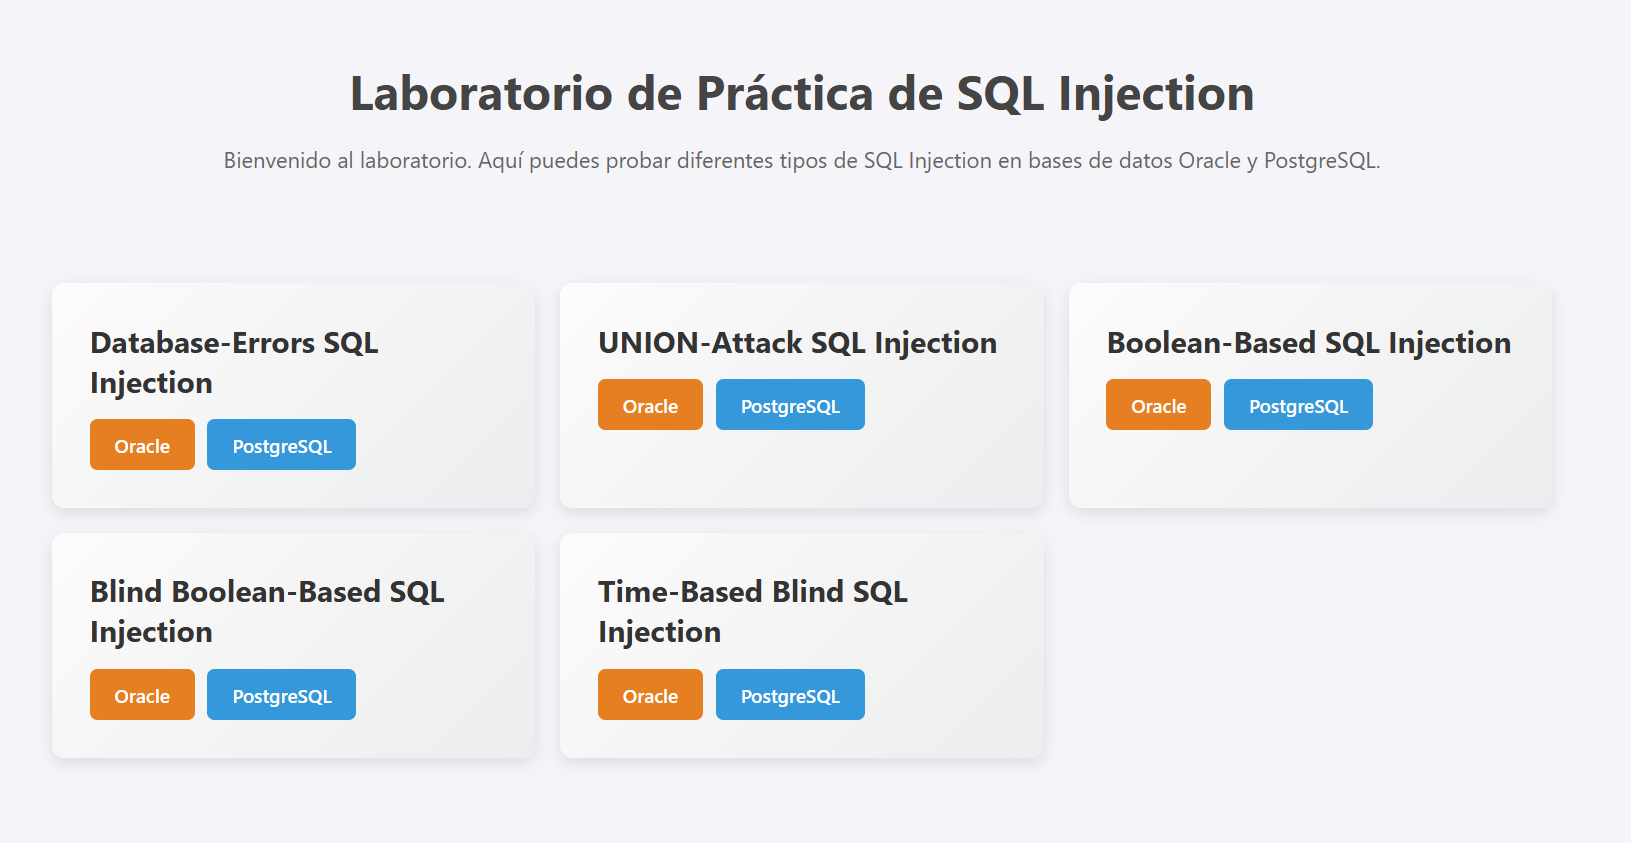
\includegraphics[width=0.8\textwidth]{Imagenes/MenuPrincipalLaboratorio.png}
    \caption{Página de inicio del laboratorio de inyecciones SQL}
\end{figure}

\section(Inyección basada en Union Attack)
La inyección SQL basada en \textbf{UNION} es una técnica en la que un atacante utiliza la cláusula UNION para combinar los resultados de una consulta legítima con datos maliciosamente solicitados, permitiendo extraer información sensible de la base de datos. 
Para llevar a cabo este ataque, el atacante identifica puntos vulnerables en la aplicación web, determina el \textbf{número de columnas} en la consulta original y luego inyecta una consulta maliciosa que utiliza \textbf{UNION SELECT} para unir los resultados deseados. 
Para prevenir este tipo de ataques, es esencial validar y sanear todas las entradas de usuario, utilizar consultas parametrizadas y aplicar el principio de privilegios mínimos en las cuentas de la base de datos.

\subsection{Proceso del ataque}

\begin{enumerate}
    \item \textbf{Identificación de puntos vulnerables:} El atacante busca parámetros de entrada en la aplicación web que interactúan directamente con la base de datos. Esto puede incluir campos de formularios, parámetros en la URL, cookies o encabezados HTTP.
    
    \item \textbf{Determinación del número de columnas:} Utilizando inyecciones como \texttt{ORDER BY} o consultas de prueba con \texttt{UNION SELECT NULL}, el atacante descubre el número de columnas en la consulta original. Esto asegura que la consulta maliciosa inyectada sea compatible con la estructura de la consulta legítima.
    
    \item \textbf{Construcción de la inyección:} Una vez identificados los parámetros vulnerables y el número de columnas, el atacante construye una consulta maliciosa utilizando \texttt{UNION SELECT}. Por ejemplo: \textit{http://example.com/page.php?id=1 UNION SELECT username, password FROM users}. En este caso, los datos sensibles de la tabla \texttt{users} son combinados con la consulta original.
\end{enumerate}

Para acceder a la sección especifica para esta inyección en el laboratorio, una vez desplegado el servidor, se 

%Conclusiones
%Anexo (Cajon desastre para codigo completo, ejecuciones completas, etc)
%Bibliografia (PortSwigger, OWASP, etc)

\end{document}
